\chapter{Measuring Tool}
A critical part of performance testing is to ensure as few variables as possible change during each run of the experiment. This generates more consistent results, and allows easier comparison between test runs.\\
In a typical science experiment setup, the variables are separated into dependent, independent, and controlled variables. The dependent variables for this testing are of course the throughput and latency numbers that result from performance benchmarking, as well as the CPU usage of the applications during the test runs. For independent variables, the implementation of the application: in node.js or Java. The exact same tests are running against different implementations. Besides these variables, everything else is controlled and kept static.\\


\section{Average Response time & Throughput}
The Average Response Time takes into consideration every round trip.The resulting metric is a reflection of the speed of the web application being tested – the best indicator of how the server is performing from the users’ perspective. The Average Response Time includes the delivery all resource being used. Thus, the average will be significantly affected by any slow components. For example,  geographic locations can have small impact on response times if the end user is thousands of miles away from the server.\\
In the thesis response time is measured in three different places as you can see from figure \ref{measure-rt} , response time is measured from three different places. The first measuring is done by load generator which records the true end-to-end time and throughput. The second checkpoint is the response time retrieved from log stash which present the round trip from router. Last measuring spot is inside server itself. It reflects the round trip of a query in database. The end-to-end measuring result is used in the final performance analysis while the others served as tool to determine where is the bottleneck of the performance test is. \\

\begin{figure}[h]
	\centering
	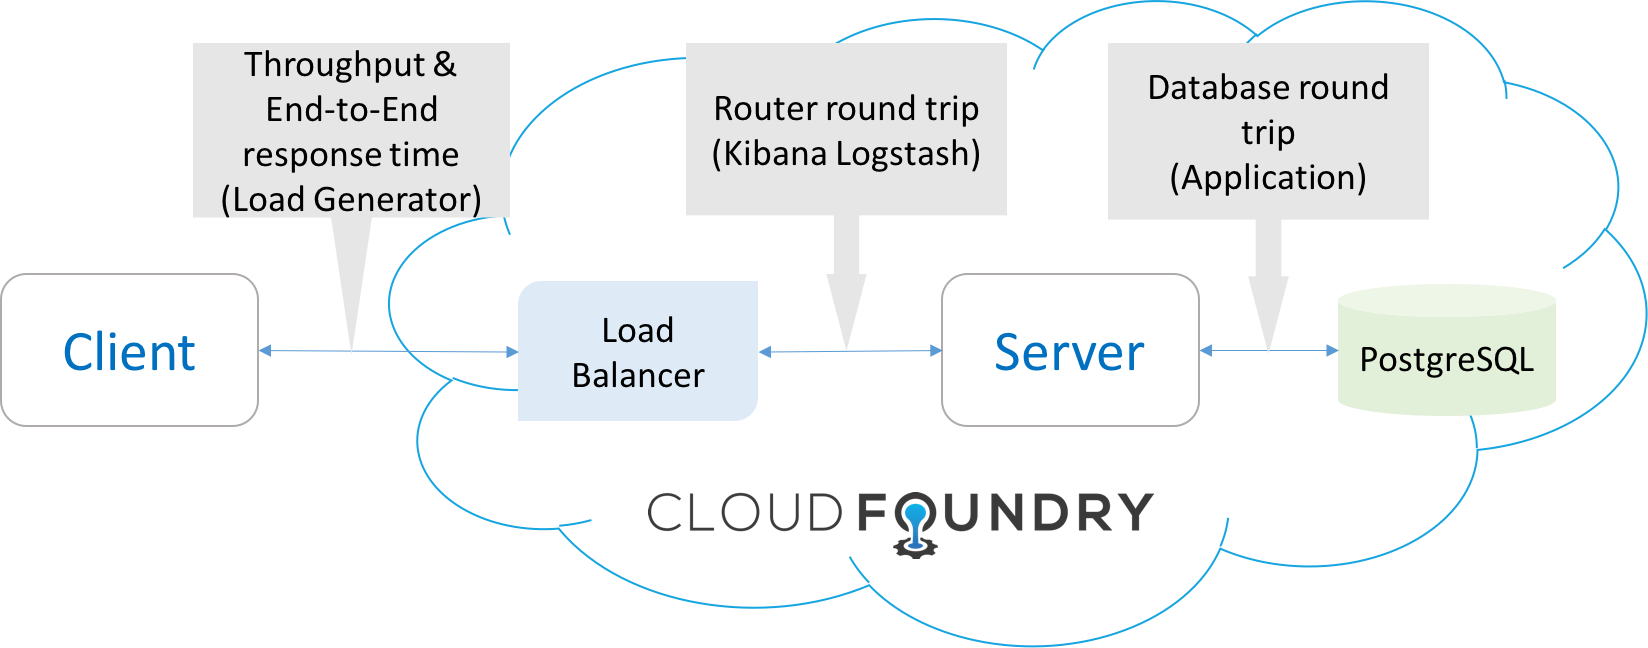
\includegraphics[width=12cm]{measure-rt}
	\caption{Measure response time three different places}
	\label{measure-rt}
\end{figure}

Throughput is the measurement of bandwidth consumed during the test. It shows how much data is flowing back and forth from servers. The requests made to the server in the thesis do not consume data of any significant size, like images. Therefore the throughput would directly reflect successfully handled amount of requests during the load testing. \\
\subsection{Recording with Load Generator and its limitations}
 In chapter \ref{load generator}, it is discussed how the load generator drives loads. It carries another duty to record the end-to-end response time fro each request. Together with response time it also stores the correlation id and start time for each request. The data is first saved in an array and insert into database at the end of load generating. \\
 However, these information are not enough. It would also be great to know the response time is resulted from which test settings, like how many application instances or how many parallel requests are sent. Therefore these information is given to the load generator and saved along with response time. Since the load generator in this thesis is only a worker, it has no API to call and set parameters. All the information external from the generator has to be given as start command. However, in cloud foundry, one application has only one start command. This means the generator should be pushed to the cloud foundry every time the parameter is changed. A small shell script is written to fulfill the task of pushing owing to the limited time frame of the thesis. \\
 It is easy to scale load generator according to what one needs. On the other hand, it also means the generator has to stay stateless, which causes some extra work. For example, the same tests may be carried out in several rounds. The result of different round should be saved to compare with each other. Making \textit{test round }a automatically incremented data type is what first comes to mind. Yet it can't be defined like that when there are more than one instance of the generator running. This parameter is hence manually given for every new round of test.\\
 
\subsection{Retrieving data from Log Stash and its limitations}
As discussed in 
  \todo[inline]{Write ELK node application and log quota}
  \subsection{Recording data inside the application and its limitations}
  \todo[inline]{Write recording data inside the application }
\section{CPU and Memory consumption}
  \todo[inline]{Write why care about cpu and memory}
\subsection{Cloud Foundry CLI and its limitations}
  \todo[inline]{Write: cf statistics}
\subsection{A self-implemented  Ruby application and its limitations}
  \todo[inline]{Do I need it?}


